 
\section{Generating a subspace of determinants}
\alert{
duplicates are avoided by checking connection to the past \\
******** (ptet exemple avec generator\_CAS versus generator\_full PSI is filtered with different function and supplied to the module using cas\_sd ( cas\_sd, mrcc ) or full\_ci ( pt2 stoch ) )?? \\
================
}

Generally speaking, a subspace of determinants is defined by a reference and a class of excitation applied to it.
\alert{
Because of the determinant-driven approach, it may not be possible to store all the determinants of the considered subspace. \textbf{Pourquoi c'est lie au determinant-driven?}
}



\paragraph{Reference space}
The \QP allows to define either a determinants of a CAS (Complete Active Space) or the full-CI space as the reference.\footnote{Although the full-CI space is a particular CAS, it is treated differently at the code level.}

\paragraph{Excitation class}
The excitations to be applied to determinants of the reference space are defined by sets of orbitals describing:
\begin{itemize}
\item
Single excitations
\item
The first excitation of a double excitation
\item
The second excitation of a double excitation
\end{itemize}
For each set category, there is one set for the allowed holes and one set for the allowed particles.
This defines the rules used to generate determinants of the external space from the reference determinants.

Typically, to define a CAS-SD (CAS augmented with all single and double excitations applied to all the determinants of the CAS), one defines:
\begin{description}
\item [Core orbitals:]
Orbitals always doubly occupied. They are not part of any of the sets.
\item [Inactive orbitals:]
Orbitals in which one or two holes may be created. They are part of the all the \emph{hole} sets.
\item [Active orbitals:]
Orbitals defining the CAS. They are part of all the sets.
\item [Virtual orbitals:]
Orbitals in which one or two particles may be created. They are part of the all the \emph{particle} sets.
\item [Deleted orbitals:]
Orbitals removed from the calculation, always unoccupied. They are not part of any set.
\end{description}


 As will be seen later, determinants are selected iteratively. The general procedure is shown 



\begin{algorithm}
        \caption{GENERAL\_SELECTION}    
        \label{alg:GENERAL_SELECTION}   
        $\ket{\Psi} \gets \ket{\HF}$\;
        Build the sets $\set{H}_0, \set{H}_1, \set{H}_2, \set{P}_0, \set{P}_1, \set{P}_2$ \;
        $\set{T}$: the set of excitations allowed on the reference based on $\set{H}_0, \set{H}_1, \set{H}_2, \set{P}_0, \set{P}_1, \set{P}_2$ \;
        
        \While{some condition}{
                $\set{D}$: the set of determinants in $\ket{\Psi}$ \;
                $\set{D}' \gets \{ \}$ \;
                \For{$i \gets 1, \Ndet$}{
                        \ForAll{$\hat{T}_j \in \set{T}$}{
                                $\kalpha \gets \ordering \hat{T}_j \ket {D_i}$ \;
                \If{$\kalpha \neq 0$}{
                /* Check if $\kalpha$ was not already generated before */ \;
                \textit{found} $\gets$ False \;
                \For{$l \gets 1, i-1$}{
                        \ForAll{$\hat{T}_k \in \set{T}$}{
                                $\textit{found} \gets \ior{\textit{found}}
            {(\ordering \hat{T}_k \ket{D_{l}} \neq \kalpha)}$ \;
                                }
                                }
                \If{$\iand{(\neg \textit{found})}{\textit{Selection\_criterion}}$ }{
                $\set{D}' \gets \set{D}' \cup \kalpha $ \;                      
                }
                                }
                        }
                }
                do some selection in $\set{D}'$ \;
                add selected determinants to $\set{D}$ \;
                diagonalize $\hat{H}$ in $\set{D}$ to obtain $\ket{\Psi}$ \;
        }
\end{algorithm}




\section{excitation driven(?) - (TOTO, INUTILE DE LIRE) a reecrire/tester}

There is a way to find connections using an 'excitation driven' approach, that would be closer to an integral-driven approach. Essentially, it is possible to find all determinants of an arbitrary set that connects by a particular excitation, with a complexity linear (logarithmic???) with $N_{det}$.
To understand this approach, we will considered bitstrings as single integers of arbitrary size.

SCHEMA


\begin{equation}
\hat T_{a}^{b} D = E
\end{equation}

\begin{equation}
ibclr(ibset(I_D, b), a)
\end{equation}
 
 
\begin{equation}
ibclr(X, a) = X - ISHFT(1,a) ; ibtest(X,a) == TRUE
\end{equation}

\begin{equation}
ibset(X, b) = X + ISHFT(1,b) ; ibtest(X,b) == FALSE
\end{equation}

If $\hat T_{a}^b$ can be applied to $D$, 
\begin{equation}
ibtest(I_D,a)\ and\ not\ ibtest(I_D,b)
\end{equation}

\begin{equation}
I_E = I_D + I_T ; I_T = ISHFT(1,b) - ISHFT(1,a)
\end{equation}

As can be seen, it is possible to have an integer representation of an excitation.

\begin{equation}
TD = E \implies I_E = I_D + I_T ; E \neq 0
\end{equation}

It must be noted that, if $T$ cannot be applied to $D$, $I_E = I_D + I_T$ will, in most cases, not be a valid reprensentation of a determinant ; that is, $popcnt(I_{E_\alpha}) \neq N_{e,\alpha} \vee popcnt(I_{E_\beta}) \neq N_{e,\beta}$. However, there are rare instances where this isn't true.

EXEMPLE avec 8bit?

Therefore, if $I_E - I_D = I_T$, additional checks are required to establish that $TD = E$.


Implementing this in Fortran may not looks straightforward considering in this language, integers are always signed, thus the leftmost bit has a special status. However, it is actually of no relevance except when it comes to sorting, and merely changing the sorting order won't cause any malfunction.
If ``signed'' sorting is however desired, it can easily be emulated. Be $X$ and $Y$ two 64-bit integers, $u_comp$ the unsigned comparison operator (the one used by Fortran) and $s_comp$ the signed comparison operator.

\begin{equation}
s\_comp(X,Y) = u\_comp(IEOR(X,ISHFT(1,63)), IEOR(Y,ISHFT(1,63))
\end{equation}


$IEOR(X,ISHFT(1,63)$ returns $X$ with bit at position 63 flipped. Bit are indexed from 0 so bit at position 63 is the leftmost one for 64-bit integers.

The algorithm for ``excitation driven'' connection finding is detailed in algorithm XX.


\begin{comment}




\begin{algorithm}
	\caption{base functions}
		
	\SetKwFunction{FMain}{AddBigint}
	\SetKwProg{Fn}{Function}{:}{}
	
	\Fn(\tcc*[h]{co}){\FMain{some args}}{
		$overflow \gets 0$ \;
		\For{$i\gets 1,N_{int}$}{
			$may \gets IOR(I[i], J[i])$ \;
			$will \gets IAND(I[i], J[i])$ \;
			$R[i] \gets I[i] + J[i] + overflow$ \;
			$overflow \gets ISHFT(IOR(will, IAND(may, not(R[i]))), -63)$ \;
		}
	}
\end{algorithm}


\begin{algorithm}
	\caption{base functions}
		
	\SetKwFunction{FMain}{AddBigint}
	\SetKwProg{Fn}{Function}{:}{}
	
	\Fn(\tcc*[h]{co}){\FMain{some args}}{
		$i \gets 1$ \;
		$j \gets 1$ \;
		\While{$i \leq N_i \& j \leq N_Q$}{
			\For{$\sigma \gets \{\alpha, \beta\}$}{
			$overflow \gets 0$ \;
			\For{$k\gets1,N_{int}$}{
				$m \gets I_i[k,\sigma] + E[k, \sigma] + overflow$ \;
				\uIf{$m > J_j[k, \sigma]$}{
					$j \gets j+1$ \;
					cycle i,j loop \;
				}\ElseIf{$m < J_j[k, \sigma]$}{
					$i \gets i+1$ \;
					cycle i,j loop \;
				}
				$may \gets IOR(I_i[k,\sigma], E[k, \sigma])$ \;
				$will \gets IAND(I_i[k,\sigma], E[k, \sigma])$ \;
				$overflow \gets ISHFT(IOR(will, IAND(may, not(m))), -63)$ \;
			}
			}
			\If{$EXC(I_i, J_j) \leq 2$}{
				$assert(J=EI)$ \;			
			}
		}
	}
\end{algorithm}





\begin{algorithm}
	\caption{base functions}
	\label{EXCITATION_DRIVEN}
	\SetKwFunction{FMain}{EXCITATION\_DRIVEN}
	\SetKwProg{Fn}{Function}{:}{}
	
		\Fn(\tcc*[h]{A VERIFIER}){\FMain{some args}}{
		$i \gets 1$ \;
		$j \gets 1$ \;
		

		\While{$i \leq N_i \& j \leq N_Q$}{
			$aim \gets APPLY(I_i, E, ok)$ \;
			\If{$not\ ok$}{
				$i \gets i+1$ \;
				cycle \;
			}
			\While{$j \leq N_Q$}{
				\tcc{find the index of $aim$ in $J$ in the range $[j, N_Q]$. If not found, return the lowest $j$ so that $detCmp(aim, J_j) = 1$, or $N_{j}+1$ if $aim > J_{N_Q}$.}
				$j \gets find(aim, J, j, N_Q, ok)$ \;
				\If{$ok$}{
					found \;
				}
				%				$cmp \gets DetCmp(J_j, aim)$ \;
%				\uIf{$cmp = 1$}{
%					break \;
%				}\ElseIf{$cmp = 0$}{
%					found \;
%					break \;
%				}
%				$j \gets j+1$ \;
			}
		}

	}
	
			
	\SetKwFunction{FDetCmp}{DetCmp}
	\SetKwProg{Fn}{Function}{:}{}
	
	\Fn(\tcc*[h]{co}){\FDetCmp{$I$, $J$}}{
		\For{$\sigma \gets \{\alpha, \beta\}$}{
		\For{$k\gets1,N_{int}$}{
			\uIf{$I_\sigma[k] > J_\sigma[k]$}{
				\KwRet{1} \;
			}\uElseIf{$I_\sigma[k] < J_\sigma[k]$}{
				\KwRet{-1} \;
			}
		}
		}
		\KwRet 0 \;
	}
\end{algorithm}
\end{comment}



\begin{algorithm}
	\caption{EXCITATION\_DRIVEN}
	\label{EXCITATION_DRIVEN}
	\SetKwFunction{FMain}{EXCITATION\_DRIVEN}
	\SetKwProg{Fn}{Function}{:}{}
	
		\Fn(\tcc*[h]{CHECK}){\FMain{$I$, $J$}}{
		$i \gets 1$ \;
		$j \gets 1$ \;
		

		\While{$i \leq N_I \& j \leq N_J$}{
			$aim \gets APPLY(I_i, E, ok)$ \;
			$j \gets find\_first\_geq(aim, J, j, N_Q, match)$ \;				
			
			\If{$not(match) \& j \leq N_Q$}{
				$aim \gets REVERSE\_APPLY(J_j, E, ok)$ \;
				$i \gets find\_first\_geq(aim, I, i, N_i, match)$ \;
				
			}
			\If{$match$}{
				\If{$ok$}{
					assert $J_j = \hat EI_i$ \;	
				}
				$i \gets i+1$ \;
			}
		}
	}

	
	
			
	\SetKwFunction{FDetCmp}{DetCmp}
	\SetKwProg{Fn}{Function}{:}{}
	
	\Fn(\tcc*[h]{REPLACE WITH find\_first\_geq}){\FDetCmp{$I$, $J$}}{
		\For{$\sigma \gets \{\alpha, \beta\}$}{
		\For{$k\gets1,N_{int}$}{
			\uIf{$I_\sigma[k] > J_\sigma[k]$}{
				\KwRet{1} \;
			}\uElseIf{$I_\sigma[k] < J_\sigma[k]$}{
				\KwRet{-1} \;
			}
		}
		}
		\KwRet 0 \;
	}
\end{algorithm}



\begin{equation}
(ij \rightarrow kl) = \big [(ij|kl) - (ij|lk) \big ] \times phase(S,ijkl)
\end{equation}


\begin{equation}
(i\bar j \rightarrow k\bar l) = (i\bar j|k\bar l) \times phase(S,i\bar jk\bar l)
\end{equation}




\begin{equation}
phase(S,ijkl) = P^S_i \oplus P^S_j \oplus P^S_{k+1} \oplus P^S_{l+1} \oplus (min(k,l)>max(i,j))
\end{equation}


\begin{equation}
phase(S,i\bar jk\bar l) = P^S_i \oplus P^S_{\bar j} \oplus P^S_{k+1} \oplus P^S_{\bar l+1}
\end{equation}



\begin{algorithm}
	\KwData{$I[]$ the children of $\kI$}
	
	\ForAll{$\ket {G_p}$ singly ionized generator}{
		\tcc{indexed by 1 hole and 2 particles}
		$c_\alpha[h,p1,p2]$ \;
		\tcc{$\kalpha \gets a_h a^\dagger_{p1} a^\dagger_{p2} \ket {G_p}$}
		\ForAll{$I,I[r],I[s]$}{
			$\alpha \gets I \oplus I[r] \oplus I[s]$ \;
			\tcc{check $||\alpha||$ ?}
			$x \gets G_p \oplus \alpha$ \;
			\If{$||x|| = 3$}{
				$(h,p1,p2) \gets \texttt{BITSTRING\_TO\_LIST}(x)$ \;
				increment $c_\alpha[h,p1,p2]$ \;		
			}
		}
	}
\end{algorithm}




\begin{algorithm}
	\label{BUILD_MICROLIST}
	\caption{BUILD\_MICROLIST}
		\KwData{ ------}
		\KwResult{ ------}
        $N \gets 0$ \;
        $N^* \gets 0$ \;   
        $N^{*,*} \gets 0$ \;    
        \ForAll{$I \in \{S - past\} ; f_{G_{pq}}^I \leq 4$}{
          $(P,H) \gets particles\_and\_holes(G_{pq}, I)$ \;
          $p \gets list\_from\_bitstring(P)$ \;
          
          %$h \gets LIST_FROM_BITSTRING(H)$
          \uIf{$f_{G_{pq}}^I = 4$ \& $B_{p_1,p_2}$}{
            $i \gets N^{p_1, p_2}+1$ \;
            $N^{p_1, p_2} \gets i$ \;
            $D^{p_1, p_2}_{i} \gets I$ \;
          }
          \uElseIf{$f_{G_{pq}}^I = 3$ \& $B_{p_1}$}{
            $i \gets N^{p_1}+1$ \;
            $N^{p_1} \gets i$ \;
            $D^{p_1}_{i} \gets I$ \;
          }
          \Else{
            $i \gets N+1$ \;
            $N \gets i$ \;
            $D_{i} \gets I$ \;
          }
        }
\end{algorithm}


\begin{comment}
\begin{algorithm}
	\caption{Build $\mathcal{C}_{rs}$ from $\tilde{\mathcal{C}}_{rs}$}
	\label{alg:compute_connected}
	\tcc{This takes place after $\tilde{\mathcal{C}}_{rs}$ and $B_{rs}$ for a given batch have been fully computed}
		\KwData{$\tilde{\mathcal{C}}_{rs}$ the intermediate sets, $B_{rs}$ the tag matrix}
		%\KwResult{$Z^\star(\Gpqrs, \mathcal{C}_{rs})$ is called for all $\Gpqrs$ of $G_{pq}$ batch that are unique $\kalpha$}
		\KwResult{$\mathcal{C}_{rs}$ is computed for all $\Gpqrs$ of $G_{pq}$ batch that are unique $\kalpha$}
        $i_1 \gets N$ \;   
        $L_{1..i_1} \gets D_{1..{i_1}}$ \;
		\tcc {$B_{r0} = FALSE$ if column entirely tagged}		
		\ForAll{$r ; B_{r0}$}{
		  $i_2 \gets i_1 + N^r$ \;
		  $L_{i_1+1..i_2} \gets D^r_{1..N^r}$ \;
		  \For{$i\gets1,N_r$}{
		    $T_{D^r_i} \gets FALSE$
		  }
		  \alert{est-ce que $B_{rr}$ est tage?} \;
		  \ForAll{$s \neq r ; B_{rs}$}{
		    $i_3 \gets i_2$ \;
		    \For{$i\gets1,N_s$}{
		      \If{$T_{D^s_i}$}{
		        $i_3 \gets i_3+1$ \;
		        $L_{i_3} \gets D^s_i$ \;
		      }
		    }
		    
		    $i_4 \gets i_3 + N^{rs}$ \;
		    $L_{i_3+1 .. i_4} \gets D^{rs}_{1..N^{rs}}$ \;
		    \tcc{$L$ is the list of all $I \in \Psi ; EXC(I, a^\dagger_r a^\dagger_s G_{pq} ) \leq 2$}
		  }
		 \For{$i\gets1,N_s$}{
		    $T_{D^r_i} \gets TRUE$
		  }
		}
\end{algorithm}
\end{comment}




\section{Generating a subspace of determinants}
\alert{
duplicates are avoided by checking connection to the past \\
******** (ptet exemple avec generator\_CAS versus generator\_full PSI is filtered with different function and supplied to the module using cas\_sd ( cas\_sd, mrcc ) or full\_ci ( pt2 stoch ) )?? \\
================
}

Generally speaking, a subspace of determinants is defined by a reference and a class of excitation applied to it.
\alert{
Because of the determinant-driven approach, it may not be possible to store all the determinants of the considered ubspace. \textbf{Pourquoi c'est lie au determinant-driven?}
}



\paragraph{Reference space}
The \QP allows to define either a determinants of a CAS (Complete Active Space) or the full-CI space as the reference.\footnote{Although the full-CI space is a particular CAS, it is treated differently at the code level.}

\paragraph{Excitation class}
The excitations to be applied to determinants of the reference space are defined by sets of orbitals describing:
\begin{itemize}
\item
Single excitations
\item
The first excitation of a double excitation
\item
The second excitation of a double excitation
\end{itemize}
For each set category, there is one set for the allowed holes and one set for the allowed particles.
This defines the rules used to generate determinants of the external space from the reference determinants.

Typically, to define a CAS-SD (CAS augmented with all single and double excitations applied to all the determinants of he CAS), one defines:
\begin{description}
\item [Core orbitals:]
Orbitals always doubly occupied. They are not part of any of the sets.
\item [Inactive orbitals:]
Orbitals in which one or two holes may be created. They are part of the all the \emph{hole} sets.
\item [Active orbitals:]
Orbitals defining the CAS. They are part of all the sets.
\item [Virtual orbitals:]
Orbitals in which one or two particles may be created. They are part of the all the \emph{particle} sets.
\item [Deleted orbitals:]
Orbitals removed from the calculation, always unoccupied. They are not part of any set.
\end{description}


 As will be seen later, determinants are selected iteratively. The general procedure is shown 



\begin{algorithm}
	\caption{GENERAL\_SELECTION}	
	\label{alg:GENERAL_SELECTION}	
	$\ket{\Psi} \gets \ket{\HF}$\;
	Build the sets $\set{H}_0, \set{H}_1, \set{H}_2, \set{P}_0, \set{P}_1, \set{P}_2$ \;
	$\set{T}$: the set of excitations allowed on the reference based on $\set{H}_0, \set{H}_1, \set{H}_2, \set{P}_0, \set{P}_1, \set{P}_2$ \;
	
	\While{some condition}{
                $\set{D}$: the set of determinants in $\ket{\Psi}$ \;
                $\set{D}' \gets \{ \}$ \;
		\For{$i \gets 1, \Ndet$}{
			\ForAll{$\hat{T}_j \in \set{T}$}{
				$\kalpha \gets \ordering \hat{T}_j \ket {D_i}$ \;
                \If{$\kalpha \neq 0$}{
                /* Check if $\kalpha$ was not already generated before */ \;
                \textit{found} $\gets$ False \;
		\For{$l \gets 1, i-1$}{
			\ForAll{$\hat{T}_k \in \set{T}$}{
				$\textit{found} \gets \ior{\textit{found}}
            {(\ordering \hat{T}_k \ket{D_{l}} \neq \kalpha)}$ \;
				}
				}
                \If{$\iand{(\neg \textit{found})}{\textit{Selection\_criterion}}$ }{
		$\set{D}' \gets \set{D}' \cup \kalpha $ \;			
                }
				}
			}
		}
		do some selection in $\set{D}'$ \;
		add selected determinants to $\set{D}$ \;
		diagonalize $\hat{H}$ in $\set{D}$ to obtain $\ket{\Psi}$ \;
	}
\end{algorithm}


\begin{algorithm}
\caption{Finding connected determinants in $\ket \Psi$}
\label{alg:davidson_find_connected}
\KwData{$\{D^\alpha\}, \{D^\beta\}$~: the set of unique $\alpha$ and $\beta$ bitstrings present in $\ket \Psi$}
\KwData{$\{D^\alpha\}_{D_i^\beta}$~: the set of $\alpha$ bitstrings that are present associated with $\beta$ bitstring $D_i^\beta$ in $\ket \Psi$}
\KwData{$\{D^\beta\}_{D_i^\alpha}$ the set of $\beta$ bitstrings that are present associated with $\alpha$ bitstring $D_i^\alpha$ in $\ket \Psi$}

\tcc{The sets described above can be easily obtained by sorting the $\alpha \beta$-bitstrings of $\ket \Psi$ with ``alpha major'' and ``beta major'' order.}


\ForEach{$D_k^\alpha \in \{D^\alpha\}$}{
\ForEach{$(D_i^\beta, D_{j \geq i}^\beta) \in {\{D^\beta\}_{D_k^\alpha}}^2$}
{
\If{$\text{EXC\_DEGREE}(D_i^\beta, D_j^\beta) \leq 2$}{
        $D_i^\beta D_k^\alpha$ connected to $D_j^\beta D_k^\alpha$ by simple or double $\beta$ excitations\;
}
}
}


\ForEach{$D_k^\beta \in \{D^\beta\}$}{
\ForEach{$(D_i^\alpha, D_{j \geq i}^\alpha) \in {\{D^\alpha\}_{D_k^\beta}}^2$}
{
\If{$\text{EXC\_DEGREE}(D_i^\alpha, D_j^\alpha) \leq 2$}{
        $D_i^\alpha D_k^\beta$ connected to $D_j^\alpha D_k^\beta$ by simple or double $\alpha$ excitations\;
}
}
}

\ForEach{$(D_i^\alpha,  D_{j \geq i}^\alpha) \in {\{D^\alpha \}}^2  \; ; \; \text{EXC\_DEGREE}(D_i^\alpha, D_{j}^\alpha) = 1$}{
\ForEach{$(D_i^\beta \in {\{D^\beta}\}_{D_i^\alpha}, D_j_\beta \in {\{U^\beta}\}_{J_\alpha})$}
{
\If{$\text{EXC\_DEGREE}(D_i^\beta, J_\beta) = 1$}
{
        $D_i^\alpha D_i^\beta$ connected to $J_\alpha J_\beta$ by $\alpha\beta$ excitations\;
}
} 
}
\end{algorithm}


\begin{algorithm}
\caption{Finding connected determinants in $\ket \Psi$}
\label{alg:davidson_find_connected}
\KwData{$\{U_\alpha\}, \{U_\beta\}$~: the set of unique $\alpha$ and $\beta$ bitstrings present in $\ket \Psi$}
\KwData{$\{U_\alpha\}_{I_\beta}$ the set of $\alpha$ bitstrings that are present associated with $\beta$ bitstring $I_\beta$ in $\ket \Psi$}
\KwData{$\{U_\beta\}_{I_\alpha}$ the set of $\beta$ bitstrings that are present associated with $\alpha$ bitstring $I_\alpha$ in $\ket \Psi$}

\tcc{The sets described above can be easily obtained by sorting the $\alpha \beta$-bitstrings of $\ket \Psi$ with ``alpha major'' and ``beta major'' order.}

\ForEach{$I_\beta \in \{U_\beta \}$}{
\ForEach{$(I_\alpha, J_\alpha) \in {\{U_\alpha\}_{I_\beta}}^2$}
{
\If{$\text{EXC\_DEGREE}(I_\alpha, J_\alpha) \leq 2$}{
	$I_\alpha I_\beta$ connected to $J_\alpha I_\beta$ by simple or double $\alpha$ excitations\;
}
}
}

\ForEach{$I_\alpha \in \{U_\alpha \}$}{
\ForEach{$(I_\beta, J_\beta) \in {\{U_\beta\}_{I_\alpha}}^2$}
{
\If{$\text{EXC\_DEGREE}(I_\beta, J_\beta) \leq 2$}{
        $I_\alpha I_\beta$ connected to $I_\alpha J_\beta$ by simple or double $\beta$ excitations\;
}
}
}

\ForEach{$(I_\alpha,  J_\alpha) \in {\{U_\alpha \}}^2  \; ; \; \text{EXC\_DEGREE}(I_\alpha, J_\alpha) = 1$}{
\ForEach{$(I_\beta \in {\{U_\beta}\}_{I_\alpha}, J_\beta \in {\{U_\beta}\}_{J_\alpha})$}
{
\If{$\text{EXC\_DEGREE}(I_\beta, J_\beta) = 1$}
{
	$I_\alpha I_\beta$ connected to $J_\alpha J_\beta$ by $\alpha\beta$ excitations\;
}
} 
}
\end{algorithm}


\begin{algorithm}
\caption{Finding connected determinants in $\ket \Psi$}
\label{alg:davidson_parallel}
\KwData{See algorithm \ref{alg:davidson_find_connected}}

\ForEach{$(I_\alpha \in {\{U^\star_\alpha \}}, J_\alpha \in {\{U_\alpha \}})  \; ; \; \text{EXC\_DEGREE}(I_\alpha, J_\alpha) = 1$}{
\ForEach{$(I_\beta \in {\{U_\beta}\}_{I_\alpha}, J_\beta \in {\{U_\beta}\}_{J_\alpha})$}
{
\If{$\text{EXC\_DEGREE}(I_\beta, J_\beta) = 1$}
{
	$I_\alpha I_\beta$ connected to $J_\alpha J_\beta$ by $\alpha\beta$ excitations\;
}
} 
}
\end{algorithm}




%%%%%
The base approach to this problem is to sort, or rather classify, determinants so as to build sets that are by construction disconnected from others. Generally speaking, the set of all determinants is split in disjoint sets $S_c$, $c$ being a mathematical object of the set $\mathcal{T}$. $\mathcal{D}$ is the set of determinants. For a specific method, we have the functions
\begin{itemize}
	\item
	$C : \mathcal{D} \rightarrow \mathcal{T}$, a function that takes a determinant and returns a value in $\mathcal{T}$
	\item
	$p : \mathcal{T}^2 \rightarrow \{ \TRUE, \FALSE \}$, a function that takes a pair $(x,y) \in \mathcal{T}^2$, and returns $\FALSE$ if all the determinants of $S_x$ are disconnected to all the determinants of $S_y$, $\TRUE$ otherwise.
	\item
	$D \in S_{C(D)}$
\end{itemize}  


Although it is not formally needed, it is pretty much necessary in practice to have some comparison operator for elements of $\mathcal{T}$, so that sets can be easily formed by sorting determinants according to their respective $C(D)$. However, the choice for this operator is entirely arbitrary and doesn't affect the method, so it will not be discussed.
    
    
We can then represent the cost of computing $\mH$ using a matrix $\mathbf{M}$ of same size, where each element $M_{ij}=1$ if the corresponding element $H_{ij}$ needs to be computed, and $M_{ij}=0$ if it is known to be zero by construction.

\alert{
Theoretical representation of $\mathbf{M}$ with 3 classes of determinants $A$, $B$, and $C$, $A$ and $C$ being by construction disconnected. $H_{ij}$ elements corresponding to the white area are, by construction, known to be null. Those in the yellow area need to be computed.
}
    
\begin{figure}[h!]
	\begin{center}
		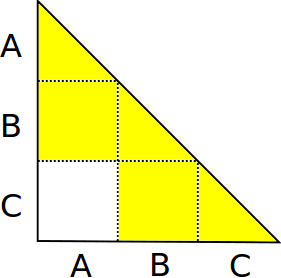
\includegraphics[width=0.4\columnwidth]{figures/davidson/disconnected_classes}
		\caption{{\label{generators_selectors}
		}}
	\end{center}
\end{figure}

Because the number of determinants used in the following examples is 500k, $M$ is shown as a density map.

As an example, one of the first attempted classification was according to the number of electrons in $s$ a subset of orbitals. Indeed, if $\ket I$ has $n$ electrons in an arbitrary subset of orbitals, and $\ket J$ has $n-3$, quite obviously it will take at least 3 excitations to excite from $\ket I$ to $\ket J$.
\begin{itemize}
	\item
	$\mathcal{T}$ is type scalar
	\item
	$C(D)$ returns the number of electrons in the chosen subset.
	\item
	$p(x, y) = |x-y| \leq 2$
\end{itemize}

Computation of $C(D)$ can be acheived using bitstrings. With $S$ a bitstring containing the orbitals wanted in the subset. The number of electrons in this subset for a determinant $\ket I$ represented by a $\alpha \beta$-bitstring $I$ is
\begin{equation}
C(I)=|I_{\alpha} \wedge S|+|I_{\beta} \wedge S|
\end{equation}

Using a subset is equivalent to using the complementary subset, so it is best to pick $N_{orb}/2$ orbitals. For a better entropy, it is of course better to interleave the chosen orbitals.
\begin{equation}
S=binary(...101010101...)
\end{equation}
    
Determinants are sorted according to this criterion. Using ClBr with 500k determinants, and sorting determinant in increasing order of their respecive $C(D)$, we got matrix $M$ shown in figure \ref{fig:num_subspace}

\begin{figure}[h!]
	\begin{center}
		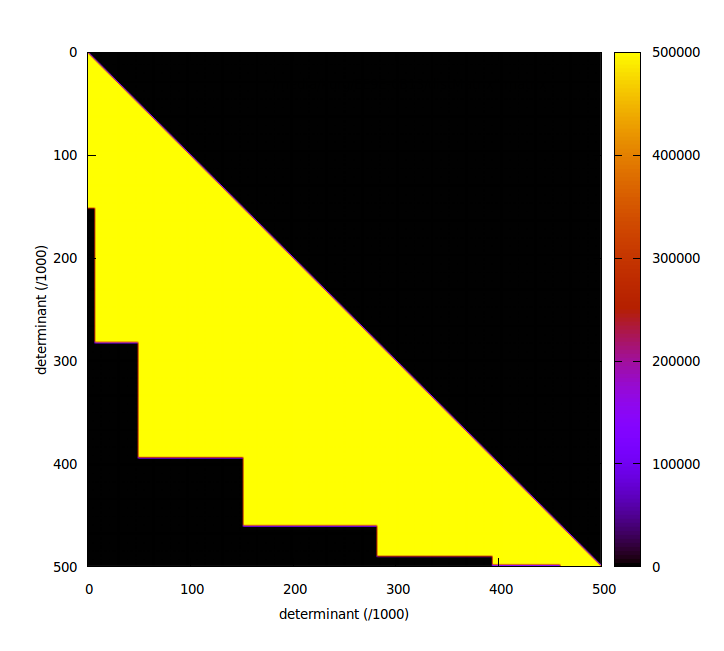
\includegraphics[width=0.6\columnwidth]{figures/davidson/num_subspace}
		\caption{{\label{fig:num_subspace}
		}}
	\end{center}
\end{figure}
    
As expected, the farther away two determinants $\ket I$ and $\ket J$ are in the sorted determinant vector, the likelier it is that $|C(I)-C(J)| > 2$ which makes them disconnected by construction. The ``staircase'' aspect shows the boundaries of each class.
However, only a relatively small area of $H$ is null by construction. It is possible to further reduce the area to be explored by chosing several orbital subsets $S_1$ to $S_n$ instead of a single one. In this case, $C(D)$ returns $c$ a vector of size $n$ with $c_{i}$ the number of electron in subset $S_i$ for $D$

\begin{itemize}
	\item
	$\mathcal{T}$ is type vector size $n$
	\item
	$C(D)$ returns $c$ a vector of size $n$, $c_i$ the number of electron in subset $S_i$
	\item
	$p(x, y) = |x_i - y_i| \leq 2 \forall i$
\end{itemize}



Using $n=3$ uncorrelated subsets
\begin{equation}
S_1 = binary(...010101010101...)
\end{equation}
\begin{equation}
S_2 = binary(...110011001100...)
\end{equation}
\begin{equation}
S_3 = binary(...111100001111...)
\end{equation}
The resulting $M$ in figure \ref{fig:num_subspace3} looks awesome but the area isn't reduced much.

\begin{figure}[h!]
	\begin{center}
		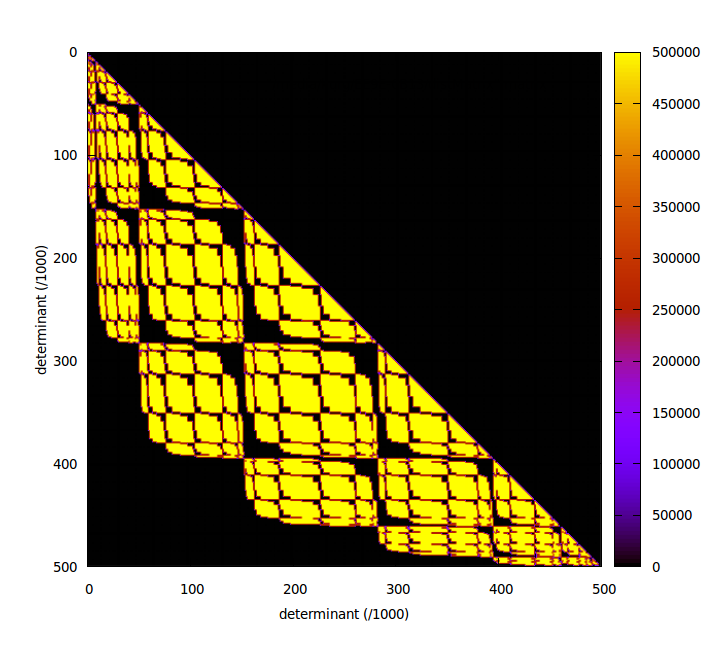
\includegraphics[width=0.6\columnwidth]{figures/davidson/num_subspace3}
		\caption{{\label{fig:num_subspace3}
		}}
	\end{center}
\end{figure}


\section{A few methods of interest}

A few methods happened to be of interest
\subsection{Highest electrons}
This method hasn't been explored throughoutly, but is still mentioned as it showed potentially interesting results, and can be use in combination with other methods.
The highest electrons are the most mobile ones, so they are the most likely not to match between two determinants. 

\begin{itemize}
	\item
$n \geq 3$ is a parameter of the method. 
	\item
$\mathcal{T}$ is a set of $n \geq 3$ electrons. 
	\item
$C(D)$ returns the set of the $n$ highest occupied spinorbitals of $D$. To make this unambiguous, it is arbitrarily decided that $\alpha$ spinorbitals are considered higher than their $\beta$ counterpart of same index.
	\item
$p(x, y) = n - |x \wedge y)| \leq 2$
\end{itemize}

$n$ is typically 3 or 4, as a larger value will result in lots of singletons, and the whole point of grouping determinants into sets being defeated. In the extreme case where $n = N_{electron}$, $C(D) = D$
   


\subsection{Singly occupied orbitals}
If there are $n$ orbitals that are singly occupied in $\ket I$ and not singly occupied in $\ket J$, it will take at least $n$ excitations to excite between $\ket I$ and $\ket J$.

\begin{itemize}
	\item
$\mathcal{T}$ is a set of orbitals
	\item
$C(D)$ returns the set of singly occupied orbitals in $D$
	\item
%$p(x, y) = max \big [popcnt(iand(x, z)), popcnt(iand(y, z)) \big ] > 2 ; z = ieor(x, y)$
$p(x, y) = max (|x|, |y|) - |x \wedge y| \leq 2$
\end{itemize}

Matrix $M$ for that method is shown in figure \ref{fig:xor_subspace}.
This method has one interesting property. If we compare determinants only with those contained in the same set - which is a tiny fraction of the total number of comparisons to be performed - we are guaranteed to find all excitations of the form $\hat T_{a \bar a}^{b \bar b}$ and $\hat T_{a \bar b}^{b \bar a}$, which are typically the largest non-diagonal matrix elements. Indeed, those excitations imply there was no change in singly occupied orbitals. And since they are the only one to do so, we are also guaranteed not to find any other type of excitation within a set.

\begin{figure}[H]
	\begin{center}
		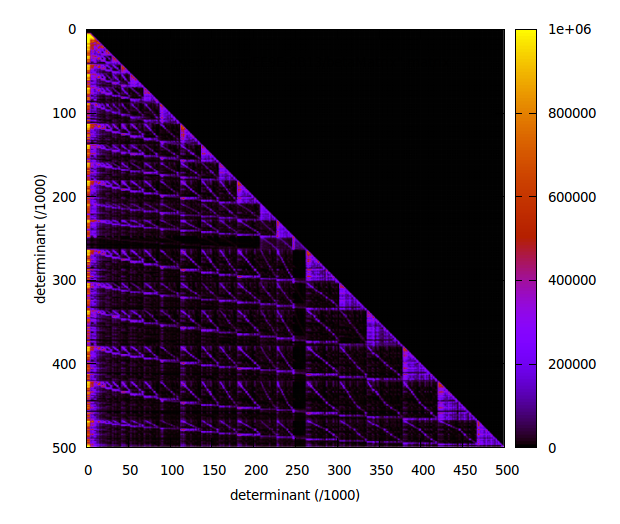
\includegraphics[width=0.6\columnwidth]{figures/davidson/xor_subspace}
		\caption{{\label{fig:xor_subspace}
		}}
	\end{center}
\end{figure}


\subsection{Simple spin part}
This methods has been implemented but was overriden by Composite spin part, introduced next. It is mostly mentioned for comprehension.

\begin{itemize}
	\item
$\mathcal{T}$ is a set of $\alpha$ spinorbitals
	\item
$C(D)$ returns $D_\alpha$, the set of occupied $\alpha$ spinorbitals in $D$
	\item
$p(x, y) = \frac{|x \oplus y|}{2} \leq 2$
\end{itemize}

$\frac{|x \oplus y|}{2}$ computes the excitation degree between $x$ and $y$ spin parts. 
    

    
\subsection{Composite spin part}
What can be noticed in the previous method, is that when we compute $p(x, y)$ to check if two sets $S_x$ and $S_y$ are disconnected, the value returned is the excitation degree for the $\alpha$ part between any $D_1 \in S_x$ and $D_2 \in S_y$. If $p(x, y)=2$, it means, $D_1$ and $D_2$ can only be connected if the excitation for the $\beta$ part is 0, in other words, if they share the same $\beta$ part. This in turn means that, when we compare determinants from $S_x$ and $S_y$, we are only looking for determinants with equal $\beta$ spin part.
Had we chosen $C(D)$ to return the $\beta$ spin part instead of the $\alpha$ one, $D_1$ and $D_2$ would have ended in the same set.
Taking this into account, we can set up a method that is made of two sub-methods, each one finding of a subset of possible excitations.

\begin{itemize}
\item
Find all connections between determinants that share the same $\alpha$ spin part. In other words, it finds all purely $\beta$ excitation,$\hat T_{\bar a}^{\bar b}$ and $\hat T_{\bar a \bar b}^{\bar c \bar d}$
\begin{itemize}
	\item
$\mathcal{T}_\alpha$ is a set of $\alpha$ spinorbitals
	\item
$C_\alpha(D)$ is the set of occupied $\alpha$ spinorbitals in $D$
	\item
%$p_\alpha(x, y) = max \big [popcnt(iand(x, z)), popcnt(iand(y, z)) \big ] > 2$, with $z = ieor(x, y)$
$p_\alpha(x, y) = (x = y)$
\end{itemize}
\item
Find all connections between determinants that are at most singly excited in their $\beta$ part.
This includes purely $\alpha$ excitation as well as $\alpha+\beta$ ones, $\hat T_a^b$, $\hat T_{ab}^{cd}$ and $\hat T_{\bar a b}^{\bar c d}$.
\begin{itemize}
	\item
$\mathcal{T}_\beta$ is a set of $\beta$ spinorbitals
	\item
$C_\beta(D)$ is the set of occupied $\beta$ spinorbitals in $D$
	\item
$p_\beta(x, y) = \frac{|x \oplus y|}{2} \leq 1$
\end{itemize}
\end{itemize}
    

All types of double excitations are found by either sub-method. The resulting $M$ matrices are shown in figures \ref{fig:aabb_subspace} and \ref{fig:ab_subspace}.
The point of this method compared to the previous one, is that the $p$ condition is drastically tightened, resulting in many more sets being by construction disconnected. For the simple spin part method, given a spin part $x$, the cardinality of the set of all $y$ spin parts so that $p(x, y) = TRUE$ is the number of possible double excitations. For composite spin part, it is respectively 1 ($p_\alpha$) and the number of single excitations ($p_\beta$).
As can be seen, the first method, although it finds all purely $\beta$ excitations, and could as well be used to find purely $\alpha$ ones, explores a minuscule area of $H$. As a matter of fact, finding those is pretty much ``free'', the vast majority of computational time is spent finding $\alpha \beta$ excitations.
As previously seen, the most important of excitations, those of the form $\hat T_{a \bar b}^{b \bar a}$, happen to be $\alpha \beta$ ones and can also be obtained for a very small cost using the singly occupied orbitals method. ( et donc? )

    
   
\begin{figure}[H]
	\begin{center}
		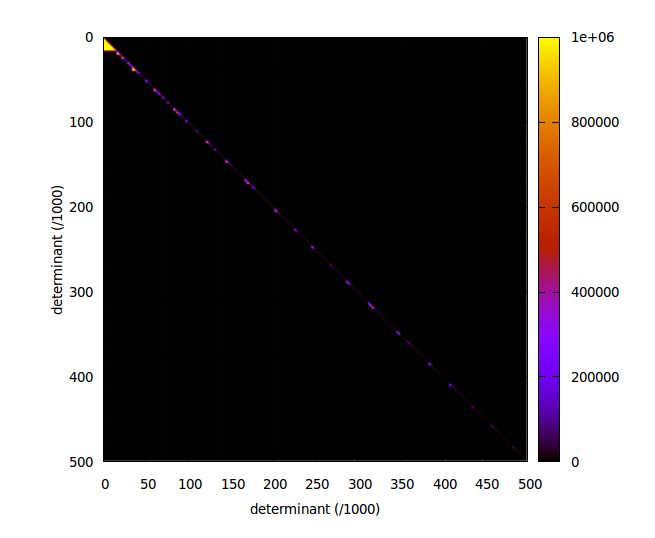
\includegraphics[width=0.6\columnwidth]{figures/davidson/aabb_subspace}
		\caption{{\label{fig:aabb_subspace}
		}}
	\end{center}
\end{figure}

\begin{figure}[H]
	\begin{center}
		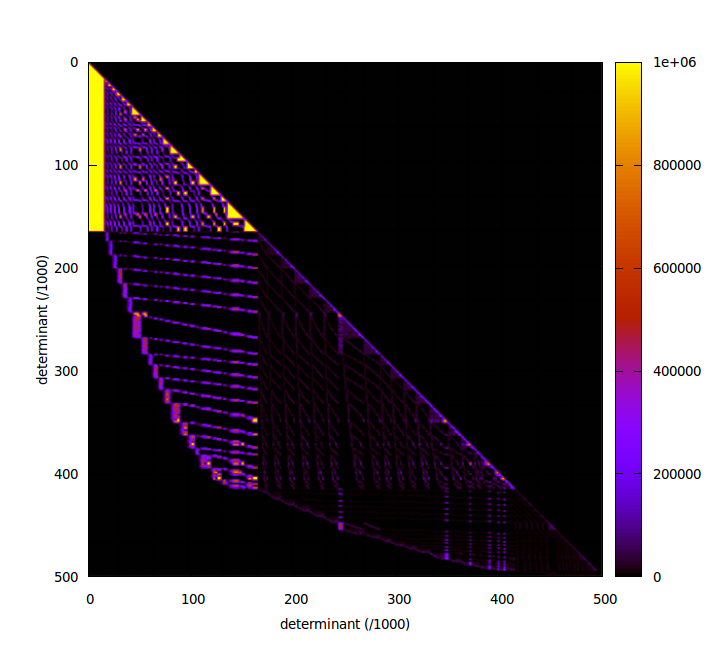
\includegraphics[width=0.55\columnwidth]{figures/davidson/ab_subspace}
		\caption{{\label{fig:ab_subspace}
		}}
	\end{center}
\end{figure}



\begin{algorithm}
	\caption{Build $\mathcal{C}_{rs}$ from $\tilde{\mathcal{C}}_{rs}$}
	\label{alg:compute_connected}
	\tcc{This takes place after $\tilde{\mathcal{C}}_{rs}$ and $B_{rs}$ for a given batch have been fully computed}
		\KwData{$\tilde{\mathcal{C}}_{rs}$ the intermediate sets, $B_{rs}$ the tag matrix}
		%\KwResult{$Z^\star(\Gpqrs, \mathcal{C}_{rs})$ is called for all $\Gpqrs$ of $G_{pq}$ batch that are unique $\kalpha$}
		\KwResult{$\mathcal{C}_{rs}$ is computed for all $\Gpqrs$ of $G_{pq}$ batch that are unique $\kalpha$} 
		\tcc{$\interC{rs}$ and $\finC{rs}$ are considered arrays, the syntax $\finC{rs}[i\ldots j]$ is used to denote a segment of array, $|\finC{rs}|$ is the cardinality of $\finC{rs}$}
		$T$ an array of size $\Nsel$ initialized to $\TRUE$ \;
		$L$ an array of determinants size $\Nsel$ \;
        $i_1 \gets |\interC{00}|$ \;   
        $L[1 \ldots i_1] \gets \interC{00}[1 \ldots {i_1}]$ \;
        
		\tcc {$B_{r0} = \TRUE$ if column $r$ is entirely tagged}		
		\ForAll{$r ; \neg B_{r0}$}{
		  $i_2 \gets i_1 + |\interC{r0}|$ \;
		  $L[i_1+1 \ldots i_2] \gets \interC{r0}$ \;
		  \For{$i\gets 1,|\interC{r0}|$}{
		    $T[\interC{r0}[i]] \gets \FALSE$
		  }
		  \ForAll{$s;\neg (B_{rs} \vee B_{0s})$}{
		    $i_3 \gets i_2$ \;
		    \For{$i\gets 1,|\interC{s0}|$}{
		      \If{$T[\interC{s0}[i]]$}{
		        $i_3 \gets i_3+1$ \;
		        $L[i_3] \gets \interC{s0}[i]$ \;
		      }
		    }
		    
		    $i_4 \gets i_3 + |\interC{rs}|$ \;
		    $L[i_3+1 .. i_4] \gets \interC{rs}$ \;
		    assert $L = \finC{rs}$
		  }
		 \For{$i\gets 1,|\interC{s0}|$}{
		    $T[\interC{s0}[i]] \gets \TRUE$
		  }
		}
\end{algorithm}

\begin{comment}
But just like for the general algorithm, if we consider $\hat T_{i'}^{j'}$ we need to sort $i'$ and $j'$ to get the $i=\min(i', j')$ and $j=\max(i', j')$ indices used for the phase computation.

This however doesn't need to be done explicitly. 




We can arbitrarily choose $i=i'$ and $j=j'$, and reverse the phase if $j<i$. We effectively have computed $p(N^I_{i'j'})$ instead of $p(N^I_{j'i'})$, and it can be proved they are always of different parity:
\begin{align}
N^{I}_{i' j'} + N^{I}_{j'i'} & = E^{I}_{j'-1} - E^I_{i'} + E^I_{i'-1} - E^I_{j'} \\
& = -\qty( \occ{j'}{I} + \occ{i'}{I})
\end{align}
Because $\hat T_{i'}^{j'} \ket I \neq 0$, we know that $\occ{j'}{I} + \occ{i'}{I} = 1$. 
\begin{equation}
N^{I}_{j' i'} = -(N^{I}_{i'j'} + 1)
\end{equation}
This translates to $N^{I}_{j' i'}$ and $N^{I}_{i'j'}$ being of different parity.

\end{comment}
